%%%%%%%%%%%%%%%%%%%%%%%%%%%%%%%%%%%%%%%%%%%%%%%%%%%%%%%%%%%%%%%%%%%%%%%%%%%

\documentclass[a4paper,oneside,12pt]{article}
\usepackage{mystyle}

\begin{document}

\title{\Large\bf Approximate $\pi$}
\author{%%
  Minh Van Nguyen \\
  \url{mvngu@gmx.com}
}
\date{\today}
\maketitle


%%%%%%%%%%%%%%%%%%%%%%%%%%%%%%%%%%%%%%%%%%%%%%%%%%%%%%%%%%%%%%%%%%%%%%%%%%%

\section{The number $\pi$}

The number $\pi = 3.141592\dots$ is a famous example of an irrational
number.  The number $\pi$ is often used to measure the area and
circumference of a circle; see \Figure{fig:general_circle}.  Since
$\pi$ is irrational, the number cannot be written as a ratio of
integers.  So for practical purposes, you must approximate $\pi$ as
closely as you can.  The Greek mathematician Archimedes used the
fraction $22 / 7$ to approximate $\pi$.  The fraction $22 / 7$ can be
written as $22 / 7 \approx 3.142857$, correct to six decimal digits.
(The symbol ``$\approx$'' means ``approximately''.)  This is not a
good approximation of $\pi$ because the value of $22 / 7$ differs from
$\pi$ from the third decimal digit onwards.  If a number $p \in \RR$
is to be a good approximation of $\pi$, then it should be possible to
make $p$ as close to $\pi$ as you want.

\begin{figure}[!htbp]
\centering
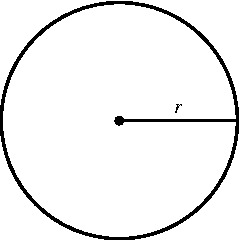
\includegraphics[scale=1]{image/05/circle.pdf}
\caption{%%
  A circle with radius $r$.  Since the radius cannot be negative, you
  must have $r \geq 0$.  The \emph{radius} of a circle is defined as
  the distance from the centre of the circle to any point on the
  circle.  The \emph{diameter}, denoted $d$, is then defined as twice
  the radius, i.e.~$d = 2r$.  The distance around the circle is called
  its \emph{circumference}.
}
\label{fig:general_circle}
\end{figure}

In order to approximate $\pi$ as closely as possible, you must know
how $\pi$ is defined.  Let $c$ be the circumference of a circle and
let $d$ be the diameter of the same circle.  Then the value of $\pi$
is defined as the ratio
%%
\begin{equation}
\label{eqn:define_pi_as_ratio_of_c_over_d}
\pi
=
\frac{c}{d}.
\end{equation}
%%
You already know that the diameter is equal to twice the radius.  The
only problem now is:
%%
\begin{packeditem}
\item How do you calculate the value of the circumference $c$?
\end{packeditem}
%%
The short answer is: You approximate the value of $c$ and then
substitute the values of $c$ and $d$ into
\Equation{eqn:define_pi_as_ratio_of_c_over_d} to obtain an
approximation of $\pi$.  What follows is the long answer.

You approximate the circumference as follows.  Draw a unit circle,
which is a circle whose radius is one unit.  Within the unit circle,
you draw a \emph{regular polygon} of $n \geq 3$ sides, which is a
shape whose $n$ sides all have equal length.  For example, an
equilateral triangle is a regular polygon with $n = 3$ sides, a square
is a regular polygon with $n = 4$ sides, and a pentagon is a regular
polygon with $n = 5$ sides.  You then use the perimeter of the regular
polygon as an approximation of the circumference of the unit circle.
A reason why this works can be seen in
\Figure{fig:unit_circle_inscribed_regular_polygon}.

\begin{figure}[!htbp]
\centering
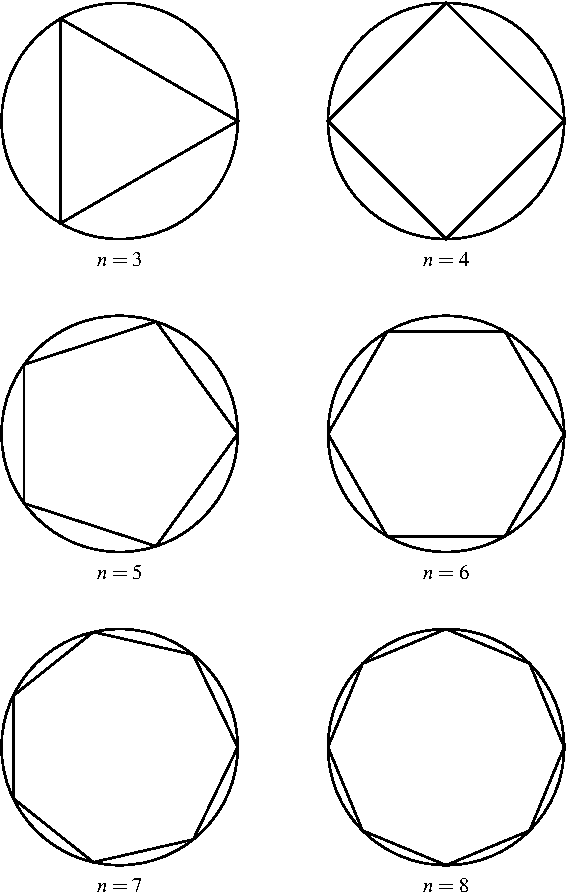
\includegraphics[scale=1]{image/05/circle-polygon.pdf}
\caption{%%
  A regular polygon inside a unit circle.  The integer $n$ is the
  number of sides of the polygon.  As the value of $n$ increases, the
  polygon looks more and more like the unit circle.
}
\label{fig:unit_circle_inscribed_regular_polygon}
\end{figure}

\begin{exercise}
Describe the circle whose radius is zero.
\end{exercise}

\ifbool{showSolution}{
\begin{solution}
The circle whose radius is zero is an infinitely small point.
\end{solution}
}{}


%%%%%%%%%%%%%%%%%%%%%%%%%%%%%%%%%%%%%%%%%%%%%%%%%%%%%%%%%%%%%%%%%%%%%%%%%%%

\section{Approximating $\pi$ with a square}

Let's start by approximating the value of $\pi$ with a square.  The
square is drawn inside a unit circle such that the four corners of the
square touch the circle; see \Figure{fig:circle_inscribed_square}.
Since the unit circle has a radius of $1$, then the unit circle has a
diameter of $d = 2$.  What remains is to approximate the circumference
$c$ of the unit circle.

\begin{figure}[!htbp]
\centering
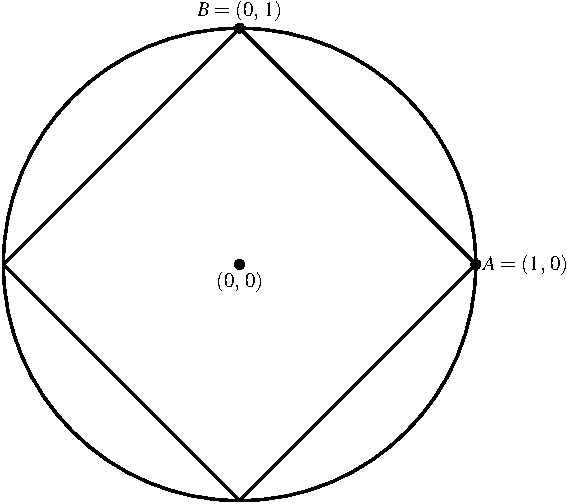
\includegraphics[scale=1.1]{image/05/circle-square.pdf}
\caption{%%
  A unit circle with an inscribed square.  A \emph{unit circle} is a
  circle whose radius is $1$.  The centre of the circle has
  coordinates $\tuple{0}{0}$.  The points $\quadruple{A}{B}{C}{D}$ are
  where the square touches the circle.  Any two neighbouring points
  are $\degree{90}$~(or $\pi / 2$ radians) apart.
}
\label{fig:circle_inscribed_square}
\end{figure}

\Figure{fig:circle_inscribed_square} suggests that the circumference
of the unit circle can be approximated by the perimeter of the
inscribed square.  If a square has a side length of $\ell$, then the
perimeter of the square is the sum of all the four sides of the
square.  In other words, the square has a perimeter of
$4\ell = \ell + \ell + \ell + \ell$.  For the square in
\Figure{fig:circle_inscribed_square} the value of $\ell$ is the length
of the line segment $AB$, which can be calculated as
%%
\begin{align*}
\ell
&=
\sqrt{(0 - 1)^2 + (1 - 0)^2} \\[4pt]
&=
\sqrt{1 + 1} \\[4pt]
&=
\sqrt{2}.
\end{align*}
%%
So the square has a perimeter of $4\ell = 4\sqrt{2}$ and you can take
this value to be an approximation of the circumference of the unit
circle.  Using \Equation{eqn:define_pi_as_ratio_of_c_over_d} you see
that the value of $\pi$ can be approximated as
%%
\begin{equation}
\label{eqn:approximate_pi_inscribed_square}
\begin{aligned}
\pi
&\approx
\frac{4\sqrt{2}}{2} \\[4pt]
&=
2\sqrt{2} \\[4pt]
&\approx
2.828427
\end{aligned}
\end{equation}
%%
correct to six decimal places.  The approximation of $2\sqrt{2}$ is
worst than Archimedes' approximate value of $22/7$.  Is there a way to
get a better approximation of $\pi$?

\begin{exercise}
Determine the area of the unit circle.
\end{exercise}

\ifbool{showSolution}{
\begin{solution}
If $r$ is the radius of a circle, then the circle has an area of
$\pi r^2$.  The unit circle has a radius of $r = 1$ so the area of the
unit circle is $\pi \times 1^2 = \pi$.
\end{solution}
}{}

\begin{exercise}
Calculate the area of the square in
\Figure{fig:circle_inscribed_square}.
\end{exercise}

\ifbool{showSolution}{
\begin{solution}
If $w$ is the width of a square, then the square has an area of
$w^2$.  As the square in \Figure{fig:circle_inscribed_square} has a
width of $\sqrt{2}$, the area of the square is $(\sqrt{2})^2 = 2$.
\end{solution}
}{}

\begin{exercise}
Let $O = \tuple{0}{0}$ be the origin.  In
\Figure{fig:circle_inscribed_square}, calculate the area of the
triangle whose corners are $\triple{O}{A}{B}$.
\end{exercise}

\ifbool{showSolution}{
\begin{solution}
The square in \Figure{fig:circle_inscribed_square} has an area of
$2$.  The area of the triangle with corners $\triple{O}{A}{B}$ is one
quarter of the area of the square.  In other words, the area of the
triangle is $2 / 4 = 1 / 2$.
\end{solution}
}{}


%%%%%%%%%%%%%%%%%%%%%%%%%%%%%%%%%%%%%%%%%%%%%%%%%%%%%%%%%%%%%%%%%%%%%%%%%%%

\section{Approximate $\pi$ with an octagon}
\label{sec:approximate_pi_with_an_octagon}

Any two neighbouring corners of the square in
\Figure{fig:circle_inscribed_square} are separated by $\pi / 2$
radians.  If you decrease the angle that separates two neighbouring
corners, then you would expect to get a better approximation to the
value of $\pi$.  In other words, you expect to get a better
approximation of $\pi$ as you increase the number of sides of the
regular polygon inside a unit circle.  Let's put the above strategy
into practice.

\begin{figure}[!htbp]
\centering
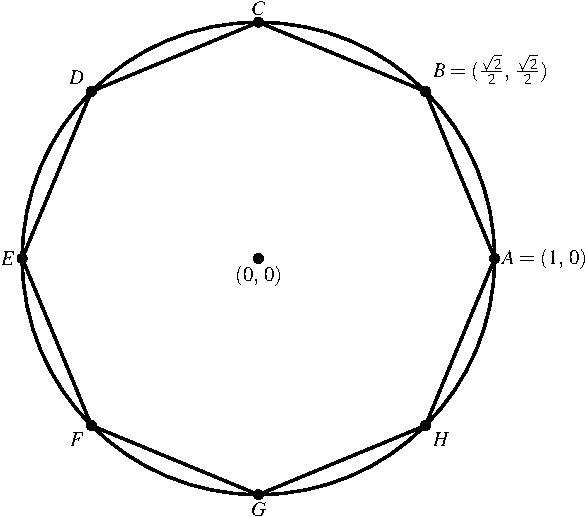
\includegraphics[scale=1]{image/05/circle-octagon.pdf}
\caption{%%
  A unit circle centred at the origin and having an inscribed
  octagon.  Except for the origin $\tuple{0}{0}$, the indicated points
  are where the octagon touches the unit circle.  Any two neighbouring
  points are $\degree{45}$~(or $\pi / 4$ radians) apart.
}
\label{fig:circle_inscribed_octagon}
\end{figure}

\Figure{fig:circle_inscribed_octagon} shows an octagon drawn inside a
unit circle.  Except for the origin $\tuple{0}{0}$, the eight labelled
points on the circle are where the octagon touches the circle.  Note
that any two neighbouring points are separated by
\[
\frac{\pi}{2} \times \frac{1}{2}
=
\frac{\pi}{4}
\]
radians.  The length of each side of the octagon is the length of the
line segment $AB$.  The distance from $A$ to $B$ is
%%
\begin{align*}
\sqrt{
  \parenthesis*{\frac{\sqrt{2}}{2} - 0}^2
  +
  \parenthesis*{\frac{\sqrt{2}}{2} - 1}^2
}
&=
\sqrt{
  \parenthesis*{\frac{\sqrt{2}}{2}}^2
  +
  \parenthesis*{\frac{\sqrt{2}}{2} - \frac{2}{2}}^2
} \\[4pt]
&=
\sqrt{
  \parenthesis*{\frac{\sqrt{2}}{2}}^2
  +
  \parenthesis*{\frac{\sqrt{2} - 2}{2}}^2
} \\[4pt]
&=
\sqrt{
  \frac{2}{4}
  +
  \frac{(\sqrt{2} - 2)^2}{4}
} \\[4pt]
&=
\sqrt{
  \frac{2}{4}
  +
  \frac{6 - 4\sqrt{2}}{4}
} \\[4pt]
&=
\sqrt{
  \frac{
    2 + 6 - 4\sqrt{2}
  }{
    4
  }
} \\[4pt]
&=
\sqrt{
  \frac{
    8 - 4\sqrt{2}
  }{
    4
  }
} \\[4pt]
&=
\sqrt{
  \frac{
    4(2 - \sqrt{2})
  }{
    4
  }
} \\[4pt]
&=
\sqrt{
  2 - \sqrt{2}
}.
\end{align*}
%%
In other words, each side of the octagon has a length of
$\ell = \sqrt{2 - \sqrt{2}}$.  Since the octagon has eight sides, then
the octagon has a perimeter of $8\ell = 8\sqrt{2 - \sqrt{2}}$ and you
can take this value to be an approximation of the circumference of the
unit circle.  Use \Equation{eqn:define_pi_as_ratio_of_c_over_d} to see
that the value of $\pi$ can be approximated as
%%
\begin{align*}
\pi
&\approx
\frac{
  8\sqrt{2 - \sqrt{2}}
}{
  2
} \\[4pt]
&=
4\sqrt{2 - \sqrt{2}} \\[4pt]
&\approx
3.061467
\end{align*}
%%
correct to six decimal places.  This is better than the
approximation~\eqref{eqn:approximate_pi_inscribed_square}, but is
worst than $22 / 7$.  You need to further decrease the angle that
separates two neighbouring points.

\begin{exercise}
In \Figure{fig:circle_inscribed_octagon}, determine the coordinates of
each point from $C$ to $H$.
\end{exercise}

\ifbool{showSolution}{
\begin{solution}
The coordinates of $C$ and $E$ are $C = \tuple{0}{1}$ and
$E = \tuple{-1}{0}$.  The point $D$ is a reflection of $B$ with
respect to the vertical axis and so
$D = (-\frac{\sqrt{2}}{2}\comma \frac{\sqrt{2}}{2})$.  Each of the
points $\triple{F}{G}{H}$ is a reflection of $\triple{D}{C}{B}$,
respectively, with respect to the horizontal axis.  Then
$F = (-\frac{\sqrt{2}}{2}\comma -\frac{\sqrt{2}}{2})$,
$G = \tuple{0}{-1}$, and
$F = (\frac{\sqrt{2}}{2}\comma -\frac{\sqrt{2}}{2})$.
\end{solution}
}{}


%%%%%%%%%%%%%%%%%%%%%%%%%%%%%%%%%%%%%%%%%%%%%%%%%%%%%%%%%%%%%%%%%%%%%%%%%%%

\section{Better approximations of $\pi$}

\Figure{fig:quadrant_inscribed_quarter_polygon_22_degrees} shows one
quarter~(or a quadrant) of a unit circle.  The arc is divided into
four equal parts, which means that the whole unit circle is divided
into $4 \times 4 = 16$ equal parts.  The distance between the points
$A$ and $B$ is
\[
\ell
=
\sqrt{
  2
  -
  \sqrt{2 + \sqrt{2}}
}
\]
and so the circumference of the unit circle can be approximated as
\[
16\ell
=
16
\sqrt{
  2
  -
  \sqrt{2 + \sqrt{2}}
}.
\]
Use \Equation{eqn:define_pi_as_ratio_of_c_over_d} to approximate $\pi$
as
%%
\begin{align*}
\pi
&\approx
\frac{
  16
  \sqrt{
    2
    -
    \sqrt{2 + \sqrt{2}}
  }
}{
  2
} \\[4pt]
&=
8
\sqrt{
  2
  -
  \sqrt{2 + \sqrt{2}}
} \\[4pt]
&\approx
3.121445
\end{align*}
%%
correct to six decimal places.  This is better than the approximation
from \Section{sec:approximate_pi_with_an_octagon}, but is worst than
$22 / 7$.

\begin{figure}[!htbp]
\centering
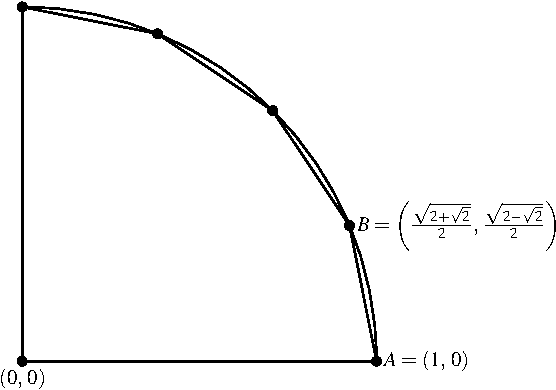
\includegraphics[scale=1.1]{image/05/quadrant.pdf}
\caption{%%
  A quadrant of the unit circle.  Inscribed in the quadrant is one
  quarter of a polygon that has $16$ sides.  The angle that separates
  two neighbouring points is $\degree{90} / 4 = \degree{22.5}$ or
  $\frac{\pi}{2} \times \frac{1}{4} = \pi / 8$ radians.
}
\label{fig:quadrant_inscribed_quarter_polygon_22_degrees}
\end{figure}

Let's generalise the above strategies for approximating the value of
$\pi$.  First, you consider a quadrant of the unit circle centred at
the origin.  Any quadrant has an angle of $\degree{90}$ or
$\pi / 2$ radians.  So you decide on an integer $k \geq 1$ to be used
for dividing $\degree{90}$.  Then the angle that separates any two
neighbouring points on the unit circle is $\pi / 2k$ radians; see
\Figure{fig:quadrant_generic_point}.  In particular, the point $B$
makes an angle of $\pi / 2k$ radians with the positive half of the
$x$-axis.

\begin{figure}[!htbp]
\centering
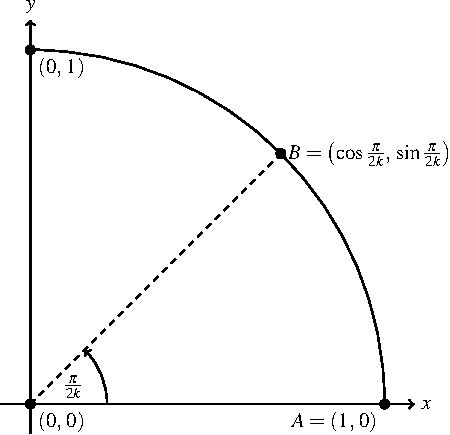
\includegraphics[scale=1.1]{image/05/quadrant-generic-point.pdf}
\caption{%%
  A quadrant of the unit circle that is centred at the origin.  The
  point $B$ on the unit circle makes an angle of $\pi / 2k$ radians
  with the positive half of the $x$-axis, where $k \geq 1$ is an
  integer.
}
\label{fig:quadrant_generic_point}
\end{figure}

Second, you calculate the length of the line segment $AB$, where
$A = \tuple{1}{0}$.  Note that the point $B$ has coordinates
$\big( \cos\frac{\pi}{2k}\comma \sin\frac{\pi}{2k} \big)$.  The
distance between $A$ and $B$ is
%%
\begin{align*}
\ell
&=
\sqrt{
  \parenthesis*{\sin\frac{\pi}{2k} - 0}^2
  +
  \parenthesis*{\cos\frac{\pi}{2k} -1}^2
} \\[4pt]
&=
\sqrt{
  \parenthesis*{\sin\frac{\pi}{2k}}^2
  +
  \parenthesis*{\cos\frac{\pi}{2k} -1}^2
} \\[4pt]
&=
\sqrt{
  2
  -
  2\cos\parenthesis*{\frac{\pi}{2k}}
}.
\end{align*}

Third, you determine the perimeter of the polygon that is drawn inside
the unit circle.  Since each quadrant is now divided into $k$ equal
parts, the whole unit circle is divided into $4k$ equal parts.  In
other words, you can draw inside the unit circle a polygon of $4k$
equal sides such that each corner of the polygon touches the unit
circle.  The polygon has a perimeter of
\[
4k\ell
=
4k\sqrt{
  2
  -
  2\cos\parenthesis*{\frac{\pi}{2k}}
}.
\]
You can use the perimeter of the polygon to approximate the
circumference of the unit circle.

Finally, you use the perimeter that you calculated above to
approximate the value of $\pi$.  Use
\Equation{eqn:define_pi_as_ratio_of_c_over_d} to approximate $\pi$ as
%%
\begin{equation}
\label{eqn:formula_approximate_pi}
\begin{aligned}
\pi
&\approx
\frac{
  4k\sqrt{
    2
    -
    2\cos\parenthesis*{\frac{\pi}{2k}}
  }
}{
  2
} \\[4pt]
&=
2k\sqrt{
  2
  -
  2\cos\parenthesis*{\frac{\pi}{2k}}
}.
\end{aligned}
\end{equation}

From \Equation{eqn:formula_approximate_pi}, you see that each specific
value of the integer $k \geq 1$ determines an approximation of the
value of $\pi$.  You would expect that as the integer $k$ gets larger
and larger, the approximation gets better and better.  Let's see if
this is the case.  For $k = 50$, \Equation{eqn:formula_approximate_pi}
gives the approximation
\[
\pi
\approx
3.14146346236400
\]
which is better than Archimedes' approximation of $22 / 7$.  For
$k = 100$, you have
\[
\pi
\approx
3.14156035548467
\]
which agrees with the first four decimal digits of $\pi$.  For
$k = 1000$, you have
\[
\pi
\approx
3.14159233062070
\]
which has the first six decimal digits of $\pi$.

\begin{exercise}
Use \Expression{eqn:formula_approximate_pi} to approximate the value
of $\pi$ for $k = \triple{1}{2}{3}$.
\end{exercise}
%%
\ifbool{showSolution}{
\begin{solution}
For $k = 1$, \Equation{eqn:formula_approximate_pi} yields the
approximation
%%
\begin{align*}
\pi
&\approx
2 \sqrt{
  2
  -
  2\cos\parenthesis*{\frac{\pi}{2}}
} \\[4pt]
&=
2 \sqrt{
  2
  -
  2 \times 0
} \\[4pt]
&=
2 \sqrt{2}
\end{align*}
%%
which can be written as $\pi \approx 2.828427$, rounded to six decimal
places.  When $k = 2$, you have the approximation
%%
\begin{align*}
\pi
&\approx
2 \times 2
\sqrt{
  2
  -
  2\cos\parenthesis*{\frac{\pi}{2 \times 2}}
} \\[4pt]
&=
4
\sqrt{
  2
  -
  2\cos\parenthesis*{\frac{\pi}{4}}
} \\[4pt]
&=
4
\sqrt{
  2
  -
  2 \times \frac{\sqrt{2}}{2}
} \\[4pt]
&=
4
\sqrt{
  2
  -
  \sqrt{2}
}
\end{align*}
%%
which can be written as $\pi \approx 3.061467$, rounded to six decimal
places.  In the case of $k = 3$, \Equation{eqn:formula_approximate_pi}
yields the approximation
%%
\begin{align*}
\pi
&\approx
2 \times 3
\sqrt{
  2
  -
  2\cos\parenthesis*{\frac{\pi}{2 \times 3}}
} \\[4pt]
&=
6
\sqrt{
  2
  -
  2\cos\parenthesis*{\frac{\pi}{6}}
} \\[4pt]
&=
6
\sqrt{
  2
  -
  2 \times \frac{\sqrt{3}}{2}
} \\[4pt]
&=
6
\sqrt{
  2
  -
  \sqrt{3}
}
\end{align*}
%%
which can be written as $\pi \approx 3.105829$, rounded to six decimal
places.
\end{solution}
}{}


\newpage
%%%%%%%%%%%%%%%%%%%%%%%%%%%%%%%%%%%%%%%%%%%%%%%%%%%%%%%%%%%%%%%%%%%%%%%%%%%

\section*{Problem}

\begin{problem}
\item Read about $\pi$ on Wikipedia or elsewhere on the Internet.
  Search for ``pi''.  Find three rational numbers that give better
  approximation of $\pi$ than $22 / 7$.
\ifbool{showSolution}{
  \begin{solution}
  The following rational numbers give better approximation of $\pi$
  than $22 / 7$:
  \[
  \frac{333}{106},
  \qquad
  \frac{355}{113},
  \qquad
  \frac{52163}{16604}.
  \]
  \end{solution}
}{}

\item Watch the following lecture on the history of $\pi$:
  \begin{center}
  \url{https://youtu.be/vVkq0KJHG6w}
  \end{center}

\item You draw a pentagon inside the unit circle such that each of the
  five corners of the pentagon touches the unit circle.  The unit
  circle is centred at the origin and each of the five sides of the
  pentagon has the same length.
  %%
  \begin{packedenum}
  \item\label{subprob:inscribed_pentagon_B_coordinates}
    Let $A = \tuple{1}{0}$ be a point on the unit circle such that $A$
    is a corner of the pentagon.  Suppose $B$ is another point on the
    unit circle such that $A$ and $B$ are neighbouring points.
    Determine the coordinates of $B$.

  \item\label{subprob:inscribed_pentagon_approximate_pi}
    The line segment $AB$ has a length of
    \[
    \ell
    =
    \sqrt{
      \frac{5 - \sqrt{5}}{2}
    }.
    \]
    Use the value of $\ell$ to approximate the value of $\pi$.
  \end{packedenum}
\ifbool{showSolution}{
  \begin{solution}
  \solutionpart{subprob:inscribed_pentagon_B_coordinates}
  The point $B$ makes an angle of $2\pi / 5$ radians with the positive
  half of the $x$-axis.  Then the coordinates of $B$ are
  $\big( \cos\frac{2\pi}{5}\comma \sin\frac{2\pi}{5} \big)$.

  \solutionpart{subprob:inscribed_pentagon_approximate_pi}
  Since the pentagon has five sides, the perimeter of the pentagon is
  \[
  5\ell
  =
  5\sqrt{
    \frac{5 - \sqrt{5}}{2}
  }
  \]
  and you can use this as an approximation of the circumference of the
  unit circle.  Now use \Equation{eqn:define_pi_as_ratio_of_c_over_d}
  to approximate $\pi$ as
  \[
  \pi
  \approx
  \frac{5}{2}
  \sqrt{
    \frac{5 - \sqrt{5}}{2}
  }.
  \]
  \end{solution}
}{}

\item A common formula for the area of a triangle is $\frac{1}{2} bh$,
  where $b$ is the length of the base of the triangle and $h$ is the
  triangle's height.  Another formula to calculate the area is
  \emph{Heron's formula}.  Heron's formula requires you to know the
  length of each side of the triangle.  Suppose that
  $\triple{a}{b}{c}$ are the lengths of the three sides of a triangle.
  Then the area of the triangle is
  \[
  \sqrt{
    s (s - a) (s - b) (s - c)
  }
  \]
  where $s$ is the fraction
  \[
  s
  =
  \frac{a + b + c}{2}.
  \]
  %%
  \begin{packedenum}
  \item\label{subprob:area_triangle_in_octagon}
    Let $O = \tuple{0}{0}$ be the origin.  In
    \Figure{fig:circle_inscribed_octagon}, compute the area of the
    triangle whose three corners are $\triple{O}{A}{B}$.

  \item\label{subprob:area_of_octagon}
    Compute the area of the octagon in
    \Figure{fig:circle_inscribed_octagon}.
  \end{packedenum}
\ifbool{showSolution}{
\begin{solution}
\solutionpart{subprob:area_triangle_in_octagon}
The line segment $AB$ has a length of $\sqrt{2 - \sqrt{2}}$.  Since
each of the points $A$ and $B$ lie on a unit circle, the distance from
$A$ to the origin~(and the distance from $B$ to the origin) is the
radius of the circle, which is $1$.  In other words, each of the line
segments $AO$ and $BO$ has a length of $1$.  Write
%%
\begin{align*}
s
&=
\frac{
  1 + 1 + \sqrt{2 - \sqrt{2}}
}{
  2
} \\[4pt]
&=
\frac{
  2 + \sqrt{2 - \sqrt{2}}
}{
  2
}.
\end{align*}
%%
Use Heron's formula to see that the triangle with corners
$\triple{O}{A}{B}$ has an area of
\[
\sqrt{
  s (s - 1) (s - 1) \parenthesis*{s - \sqrt{2 - \sqrt{2}}}
}
=
\frac{\sqrt{2}}{4}.
\]

\solutionpart{subprob:area_of_octagon}
The area of the octagon is just the area of the triangle $OAB$
repeated eight times.  Since the triangle $OAB$ has an area of
$\sqrt{2} / 4$, the area of the octagon is
%%
\begin{align*}
8 \times \frac{\sqrt{2}}{4}
&=
\frac{8 \sqrt{2}}{4} \\[4pt]
&=
2\sqrt{2}.
\end{align*}
\end{solution}
}{}

\item Read more about triangles on Wikipedia.  Determine and explain
  another formula for the area of a triangle.  The formula should be
  written in terms of the sine function.
\ifbool{showSolution}{
  \begin{solution}
  Let $a$ and $b$ be two sides of a triangle and let $\varphi$ be the
  angle~(in radians) between those two sides.  You may suppose that
  $b$ lies on the positive half of the horizontal axis and that $a$ is
  the radius of a circle centred at the origin.  Draw a straight
  vertical line from the tip of the side $a$ down to the positive half
  of the $x$-axis.  The length of the straight line is $a\sin\varphi$,
  which is also called the height of the triangle.  So $b$ is the base
  of the triangle.  Then the area of the triangle can be written as
  $\frac{1}{2} ab \sin\varphi$.
  \end{solution}
}{}

\item A unit circle is centred at the origin.  You draw a hexagon
  inside the circle such that each of the six points of the hexagon
  touches the circle.  Suppose that all sides of the hexagon have the
  same length.
  %%
  \begin{packedenum}
  \item\label{subprob:hexagon_coordinates}
    Let $A = \tuple{1}{0}$ be a corner of the hexagon.  Determine the
    coordinates of each of the remaining corners of the hexagon.

  \item\label{subprob:hexagon_area}
    Calculate the area of the hexagon.

  \item\label{subprob:hexagon_approximate_pi}
    Use the perimeter of the hexagon to approximate the value of
    $\pi$.
  \end{packedenum}
\ifbool{showSolution}{
  \begin{solution}
  \solutionpart{subprob:hexagon_coordinates}
  See \Figure{fig:inscribed_hexagon_coordinates}.
  %%
  \begin{figure}[!htbp]
  \centering
  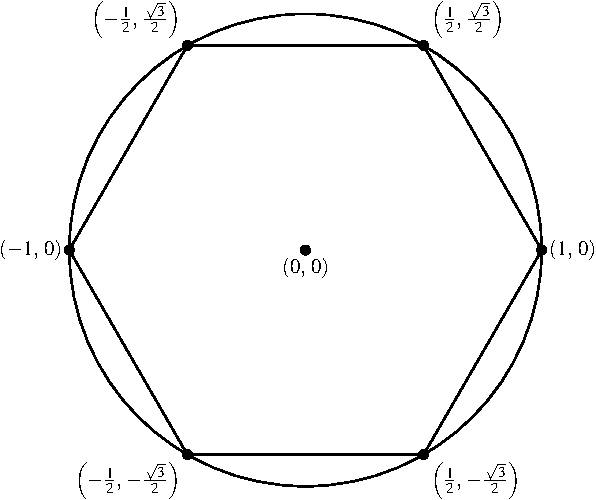
\includegraphics[scale=1.1]{image/05/circle-hexagon.pdf}
  \caption{%%
    A unit circle with an inscribed hexagon.
  }
  \label{fig:inscribed_hexagon_coordinates}
  \end{figure}

  \solutionpart{subprob:hexagon_area}
  Consider the triangle whose corners have the coordinates
  $O = \tuple{0}{0}$, $A = \tuple{1}{0}$, and
  $B = \tuple{\frac{1}{2}}{\frac{\sqrt{3}}{2}}$.  The hexagon is made
  up of six copies of this triangle.  Use Heron's formula to calculate
  the area of the triangle $OAB$ and then multiply the result by six.
  The line segment segment $OA$ has a length of $1$.  The line segment
  $AB$ has length
  %%
  \begin{align*}
  \sqrt{
    \parenthesis*{\frac{\sqrt{3}}{2} - 0}^2
    +
    \parenthesis*{\frac{1}{2} - 1}^2
  }
  &=
  \sqrt{
    \parenthesis*{\frac{\sqrt{3}}{2}}^2
    +
    \parenthesis*{-\frac{1}{2}}^2
  } \\[4pt]
  &=
  \sqrt{
    \frac{3}{4} + \frac{1}{4}
  } \\[4pt]
  &=
  1.
  \end{align*}
  %%
  The line segment $OB$ also has length $1$ because
  %%
  \begin{align*}
  \sqrt{
    \parenthesis*{\frac{\sqrt{3}}{2} - 0}^2
    +
    \parenthesis*{\frac{1}{2} - 0}^2
  }
  &=
  \sqrt{
    \parenthesis*{\frac{\sqrt{3}}{2}}^2
    +
    \parenthesis*{\frac{1}{2}}^2
  } \\[4pt]
  &=
  \sqrt{
    \frac{3}{4}
    +
    \frac{1}{4}
  } \\[4pt]
  &=
  1.
  \end{align*}
  %%
  Using Heron's formula, write $s = 3 / 2$ and so the area of the
  triangle $OAB$ is
  %%
  \begin{align*}
  \sqrt{
    s (s - 1) (s - 1) (s - 1)
  }
  &=
  \sqrt{
    \frac{3}{2} \parenthesis*{\frac{3}{2} - 1}^3
  } \\[4pt]
  &=
  \sqrt{
    \frac{3}{2} \parenthesis*{\frac{1}{2}}^3
  } \\[4pt]
  &=
  \sqrt{
    \frac{3}{2} \times \frac{1}{8}
  } \\[4pt]
  &=
  \sqrt{\frac{3}{16}} \\[4pt]
  &=
  \frac{\sqrt{3}}{\sqrt{16}} \\[4pt]
  &=
  \frac{\sqrt{3}}{4}
  \end{align*}
  %%
  Therefore the hexagon has an area of
  $\frac{6\sqrt{3}}{4} = \frac{3\sqrt{3}}{2}$.

  \solutionpart{subprob:hexagon_approximate_pi}
  From \Part{subprob:hexagon_area} you know that each side of the
  hexagon has length $1$.  Then the hexagon has a perimeter of
  $6 \times 1 = 6$, which you can use as an approximation of the
  circumference of the unit circle.  Use
  \Equation{eqn:define_pi_as_ratio_of_c_over_d} to see that the value
  of $\pi$ can be approximated as
  %%
  \begin{align*}
  \pi
  &\approx
  \frac{6}{2} \\[4pt]
  &=
  3.
  \end{align*}
  \end{solution}
}{}

\item Read more about Archimedes from the following website:
  %%
  \begin{center}
  \url{http://www-history.mcs.st-and.ac.uk}
  \end{center}
  %%
  Search for ``Archimedes''.
  %%
  \begin{packedenum}
  \item Besides mathematics, name a science that Archimedes worked
    on.

  \item Name two gadgets that Archimedes invented.

  \item Describe two books that Archimedes wrote.
  \end{packedenum}
\ifbool{showSolution}{
  \begin{solution}
  Besides mathematics, Archimedes also worked on physics.  He invented
  a screw called ``Archimedes' screw'' and a pulley called the
  ``compound pulley''.  Among Archimedes' books are
  \emph{On plane equilibriums} and \emph{On the sphere and cylinder}.
  The book \emph{On plane equilibriums} is about a branch of physics
  called mechanics.  In the book \emph{On the sphere and cylinder},
  Archimedes described several geometric properties of the sphere.
  \end{solution}
}{}

\begin{figure}[!htbp]
\centering
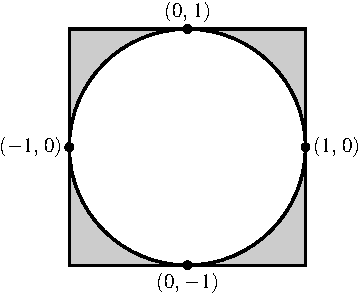
\includegraphics[scale=1]{image/05/square-inscribed-circle.pdf}
\caption{%%
  A unit circle drawn inside a square.  The unit circle touches the
  square at the given four points.  Inside the unit circle is an
  inscribed square that touches the unit circle at the given four
  points.  Finally, inside the inscribed square is an inscribed circle
  that touches the inscribed square at four points.
}
\label{fig:square_inscribed_circle}
\end{figure}

\item A unit circle is inscribed within a square as shown in
  \Figure{fig:square_inscribed_circle}.  The unit circle touches the
  square at exactly the four points shown in the figure.  Inside the
  unit circle is an inscribed square, which contains an inscribed
  circle that touches the inscribed square at four points.  Calculate
  the area of the shaded region in
  \Figure{fig:square_inscribed_circle}.
\ifbool{showSolution}{
\begin{solution}
First, consider the shaded area between the outer square and the unit
circle.  The unit circle has a radius of $r = 1$ unit so the circle
has an area of $\pi r^2 = \pi$ units.  Each side of the outer square
has a length equal to the diameter of the unit circle.  Then each side
of the outer square has a length of $2r = 2$ units so the area of the
square is $2^2 = 4$ units.  The area of the shaded region between the
outer square and the unit circle is $4 - \pi$ units.

Second, consider the shaded region between the inner square and its
inscribed circle.  Each side of the inner square has a length of
%%
\begin{align*}
\sqrt{
  (1 - 0)^2 + (0 - 1)^2
}
&=
\sqrt{
  1^2 + (-1)^2
} \\[4pt]
&=
\sqrt{2}
\end{align*}
%%
units, which is also the diameter of the inscribed inner circle.  The
area of the inner square is $(\sqrt{2})^2 = 2$ units.  The circle
within the inscribed square has a radius of $\sqrt{2} / 2$ units and
hence the inner circle has an area of
%%
\begin{align*}
\parenthesis*{\frac{\sqrt{2}}{2}}^2 \pi
&=
\frac{2}{4} \pi \\[4pt]
&=
\frac{\pi}{2}
\end{align*}
%%
units.  The shaded region between the inner square and its inscribed
circle is $2 - \frac{\pi}{2}$ units.  Therefore the area of the shaded
region in \Figure{fig:square_inscribed_circle} is
%%
\begin{align*}
(4 - \pi) + \parenthesis*{2 - \frac{\pi}{2}}
&=
4 - \pi + 2 - \frac{\pi}{2} \\[4pt]
&=
4 + 2 - \pi - \frac{\pi}{2} \\[4pt]
&=
6 - \frac{2\pi}{2} - \frac{\pi}{2} \\[4pt]
&=
6 - \frac{3\pi}{2}
\end{align*}
%%
or approximately $1.287611$ units, rounded to six decimal places.
\end{solution}
}{}

\begin{figure}[!htbp]
\centering
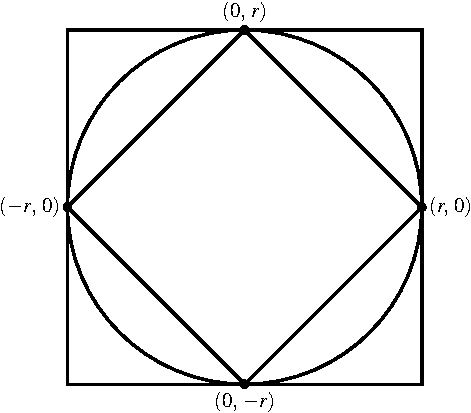
\includegraphics[scale=1]{image/05/square-circle-square.pdf}
\caption{%%
  An outer square with an inscribed circle of radius $r > 0$.  Inside
  the circle is a smaller square.
}
\label{fig:square_unit_circle_square}
\end{figure}

\item \Figure{fig:square_unit_circle_square} shows a square that has a
  circle, which in turn has a square.  The three shapes touch each
  other at the given four points.
  %%
  \begin{packedenum}
  \item\label{subprob:areas_big_square_circle_small_square}
    Let $\triple{A}{B}{C}$ be the areas of the outer square, the
    circle, and the inner square, respectively.  Explain why
    $C < B < A$.

  \item\label{subprob:bound_pi}
    Prove that $2 < \pi < 4$.
  \end{packedenum}
\ifbool{showSolution}{
\begin{solution}
\solutionpart{subprob:areas_big_square_circle_small_square}
Since the circle has a radius of $r > 0$, its diameter is $2r$ and so
the area of the outer square is $A = (2r)^2 = 4r^2$.  The circle has
an area of $B = \pi r^2$.  Each side of the inner square has a length
of
%%
\begin{align*}
\ell
&=
\sqrt{
  (r - 0)^2 + (0 - r)^2
} \\[4pt]
&=
\sqrt{
  r^2 + r^2
} \\[4pt]
&=
\sqrt{2r^2} \\[4pt]
&=
r\sqrt{2}
\end{align*}
%%
so that the inner square has an area of $C = (r\sqrt{2})^2 = 2r^2$.
The inner square is drawn inside the circle, so it must be that
$C < B$.  Furthermore, the circle is drawn inside the outer square so
it must be that $B < A$.

\solutionpart{subprob:bound_pi}
From \Part{subprob:areas_big_square_circle_small_square} you know that
$2r^2 < \pi r^2 < 4 r^2$.  Divide each term by $r^2$ to see that
$2 < \pi < 4$.
\end{solution}
}{}

\begin{figure}[!htbp]
\centering
\subfigure[]{
  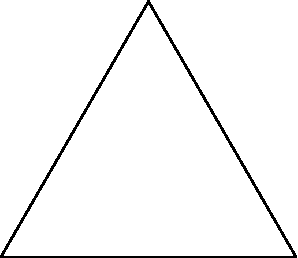
\includegraphics[scale=1]{image/05/koch-snowflake-0.pdf}
  \label{fig:Koch_snowflake_zeroth_iteration}
}
%%
\qquad
%%
\subfigure[]{
  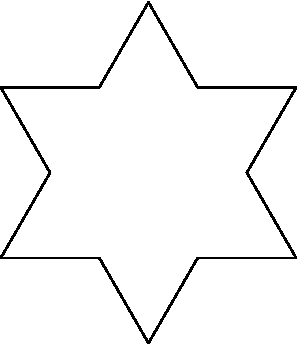
\includegraphics[scale=1]{image/05/koch-snowflake-1.pdf}
  \label{fig:Koch_snowflake_first_iteration}
} \\[4pt]
%%
%%
\subfigure[]{
  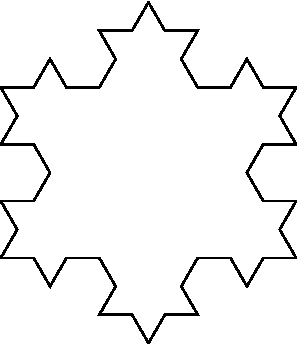
\includegraphics[scale=1]{image/05/koch-snowflake-2.pdf}
  \label{fig:Koch_snowflake_second_iteration}
}
%%
\qquad
%%
\subfigure[]{
  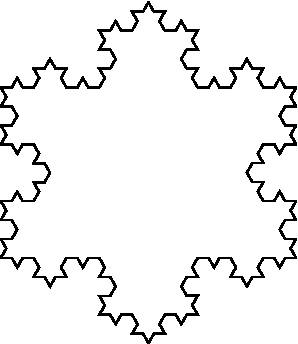
\includegraphics[scale=1]{image/05/koch-snowflake-3.pdf}
  \label{fig:Koch_snowflake_third_iteration}
}
\caption{%%
  The first four iterations of the Koch snowflake.
}
\label{fig:Koch_snowflake_first_4_iterations}
\end{figure}

\item The \emph{Koch snowflake} is a fractal curve that looks like a
  snowflake.  The construction of the Koch snowflake starts with an
  equilateral triangle.  Each line segment is modified according to
  the following rules:
  %%
  \begin{packedenumeral}
  \item Divide the line segment into three segments of equal length.
    Let $\ell$ be the middle segment.

  \item Construct an equilateral triangle whose base is $\ell$ and
    points outward.

  \item Remove the segment $\ell$.
  \end{packedenumeral}
  %%
  The starting equilateral triangle is the result of the zeroth
  iteration.  The first iteration consists of applying the above three
  rules to each line segment of the equilateral triangle.  The second
  iteration starts with the result of the first iteration and applies
  the above three rules to each line segment.  And so on; see
  \Figure{fig:Koch_snowflake_first_4_iterations}.  Suppose you start
  with an equilateral triangle each of whose three sides has length
  one.
  %%
  \begin{packedenum}
  \item\label{subprob:Koch_snowflake_zeroth_iteration}
    Calculate the perimeter and area of the shape in
    \Figure{fig:Koch_snowflake_zeroth_iteration}.

  \item\label{subprob:Koch_snowflake_first_iteration}
    Calculate the perimeter and area of the shape in
    \Figure{fig:Koch_snowflake_first_iteration}.

  \item\label{subprob:Koch_snowflake_second_iteration}
    Calculate the perimeter and area of the shape in
    \Figure{fig:Koch_snowflake_second_iteration}.
  \end{packedenum}
\ifbool{showSolution}{
\begin{solution}
\solutionpart{subprob:Koch_snowflake_zeroth_iteration}
\Figure{fig:Koch_snowflake_zeroth_iteration} is an equilateral
triangle each of whose three sides has length one.  The triangle has a
perimeter of $3$.  To calculate the area of the triangle, you can use
Heron's formula because you already know the length of each side.  By
Heron's formula, you have the value
\[
s
=
\frac{1 + 1 + 1}{2}
=
\frac{3}{2}
\]
and so the area of the triangle is given by
%%
\begin{align*}
A
&=
\sqrt{
  s (s - 1) (s - 1) (s - 1)
} \\[4pt]
&=
\sqrt{
  s (s - 1)^3
} \\[4pt]
&=
\sqrt{
  \frac{3}{2}
  \parenthesis*{\frac{3}{2} - \frac{2}{2}}^3
} \\[4pt]
&=
\sqrt{
  \frac{3}{2}
  \parenthesis*{\frac{1}{2}}^3
} \\[4pt]
&=
\sqrt{
  \frac{3}{2} \times \frac{1}{2^3}
} \\[4pt]
&=
\sqrt{
  \frac{3}{16}
} \\[4pt]
&=
\frac{\sqrt{3}}{4}.
\end{align*}

\solutionpart{subprob:Koch_snowflake_first_iteration}
To get the shape in \Figure{fig:Koch_snowflake_first_iteration}, each
line segment from the triangle of
\Figure{fig:Koch_snowflake_zeroth_iteration} was first broken up into
three segments of equal length.  In other words, each line segment of
the shape in \Figure{fig:Koch_snowflake_first_iteration} has a length
of $1/3$.  Since the shape has $12$ line segments, the perimeter of
the shape is $\frac{1}{3} \times 12 = \frac{12}{3} = 4$.

To calculate the area, note that you already know the area of the
shaded triangle in
\Figure{fig:Koch_snowflake_first_iteration_shaded_area}, which was
calculated in \Part{subprob:Koch_snowflake_zeroth_iteration}.  All you
need to do now is calculate the area of each unshaded triangle in
\Figure{fig:Koch_snowflake_first_iteration_shaded_area}.  Each of the
unshaded triangle in
\Figure{fig:Koch_snowflake_first_iteration_shaded_area} is an
equilateral triangle each of whose three sides has a length of $1/3$.
Using Heron's formula, you have the value
%%
\begin{align*}
s
&=
\frac{
  \frac{1}{3} + \frac{1}{3} + \frac{1}{3}
}{
  2
} \\[4pt]
&=
\frac{1}{2}
\end{align*}
%%
and so each unshaded triangle has an area of
%%
\begin{align*}
\sqrt{
  s \parenthesis*{s - \frac{1}{3}}^3
}
&=
\sqrt{
  \frac{1}{2} \parenthesis*{\frac{1}{2} - \frac{1}{3}}^3
} \\[4pt]
&=
\sqrt{
  \frac{1}{2} \parenthesis*{\frac{1}{6}}^3
} \\[4pt]
&=
\sqrt{
  \frac{1}{2} \times \frac{1}{(2 \times 3)^3}
} \\[4pt]
&=
\sqrt{
  \frac{1}{2^4 \times 3^3}
} \\[4pt]
&=
\frac{
  1
}{
  4 \times 3 \sqrt{3}
} \\[4pt]
&=
\frac{
  1
}{
  12 \sqrt{3}
} \\[4pt]
&=
\frac{
  1
}{
  12 \sqrt{3}
}
\times
\frac{\sqrt{3}}{\sqrt{3}} \\[4pt]
&=
\frac{
  \sqrt{3}
}{
  36
}.
\end{align*}
%%
The area of the shape in \Figure{fig:Koch_snowflake_first_iteration}
is therefore
%%
\begin{align*}
B
&=
A + 3 \times \frac{\sqrt{3}}{36} \\[4pt]
&=
\frac{\sqrt{3}}{4} + \frac{\sqrt{3}}{12} \\[4pt]
&=
\frac{\sqrt{3}}{4} \times \frac{3}{3} + \frac{\sqrt{3}}{12} \\[4pt]
&=
\frac{3\sqrt{3} + \sqrt{3}}{12} \\[4pt]
&=
\frac{4\sqrt{3}}{12} \\[4pt]
&=
\frac{\sqrt{3}}{3}.
\end{align*}
%%

\begin{figure}[!htbp]
\centering
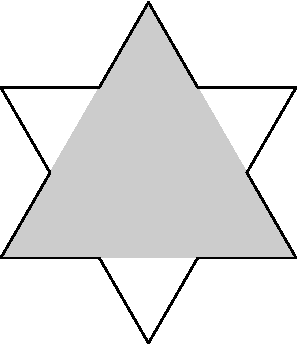
\includegraphics[scale=1]{image/05/koch-snowflake-1-area.pdf}
\caption{%%
  The first iteration of the Koch snowflake.  The shaded triangle is
  the equilateral triangle with which you started.
}
\label{fig:Koch_snowflake_first_iteration_shaded_area}
\end{figure}

\begin{figure}[!htbp]
\centering
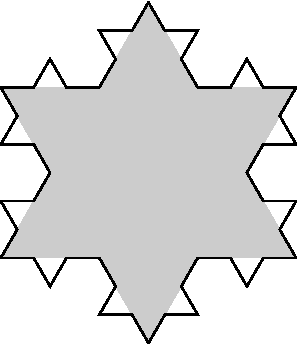
\includegraphics[scale=1]{image/05/koch-snowflake-2-area.pdf}
\caption{%%
  The second iteration of the Koch snowflake.  The shaded region is
  the shape from
  \Figure{fig:Koch_snowflake_first_iteration_shaded_area}.
}
\label{fig:Koch_snowflake_second_iteration_shaded_area}
\end{figure}

\solutionpart{subprob:Koch_snowflake_second_iteration}
The perimeter of the shape in
\Figure{fig:Koch_snowflake_second_iteration} is calculated in the same
way as you did for \Part{subprob:Koch_snowflake_first_iteration}.
Each line segment of the shape in
\Figure{fig:Koch_snowflake_second_iteration} is obtained by breaking
up each line segment from \Figure{fig:Koch_snowflake_first_iteration}
into three equal parts.  Thus each line segment in
\Figure{fig:Koch_snowflake_second_iteration} has a length of
$\frac{1}{3} \times \frac{1}{3} = \frac{1}{9}$.  As there are $48$
line segments, the shape has a perimeter of
%%
\begin{align*}
\frac{1}{9} \times 48
&=
\frac{1}{9} \times \frac{3 \times 16}{1} \\[4pt]
&=
\frac{16}{3}.
\end{align*}

To calculate the area, you do as you did
in \Part{subprob:Koch_snowflake_first_iteration}.  You already know
the area of the shaded region in
\Figure{fig:Koch_snowflake_second_iteration_shaded_area} so what
remains is to calculate the area of each unshaded triangle in
\Figure{fig:Koch_snowflake_second_iteration_shaded_area}.  Using
Heron's formula, you have the value
%%
\begin{align*}
s
&=
\frac{
  \frac{1}{9} + \frac{1}{9} + \frac{1}{9}
}{
  2
} \\[4pt]
&=
\frac{3}{9} \times \frac{1}{2} \\[4pt]
&=
\frac{1}{3} \times \frac{1}{2} \\[4pt]
&=
\frac{1}{6}
\end{align*}
%%
and so each unshaded triangle in
\Figure{fig:Koch_snowflake_second_iteration_shaded_area} has an area
of
%%
\begin{align*}
\sqrt{
  s \parenthesis*{s - \frac{1}{9}}^3
}
&=
\sqrt{
  \frac{1}{6} \parenthesis*{\frac{1}{6} - \frac{1}{9}}^3
} \\[4pt]
&=
\sqrt{
  \frac{1}{6} \parenthesis*{\frac{1}{18}}^3
} \\[4pt]
&=
\sqrt{
  \frac{1}{2 \times 3} \times \frac{1}{2^3 \times 3^6}
} \\[4pt]
&=
\sqrt{
  \frac{1}{2^4 \times 3^7}
} \\[4pt]
&=
\sqrt{
  \frac{1}{4^2 \times 9^2 \times 3^2 \times 3}
} \\[4pt]
&=
\frac{1}{
  4 \times 9 \times 3
  \sqrt{
    3
  }
} \\[4pt]
&=
\frac{1}{
  4 \times 3^3
  \sqrt{
    3
  }
} \\[4pt]
&=
\frac{1}{
  4 \times 3^3
  \sqrt{
    3
  }
}
\times
\frac{\sqrt{3}}{\sqrt{3}} \\[4pt]
&=
\frac{\sqrt{3}}{
  4 \times 3^4
}.
\end{align*}
%%
Therefore the shape in \Figure{fig:Koch_snowflake_second_iteration}
has an area of
%%
\begin{align*}
C
&=
B
+
12 \times \frac{\sqrt{3}}{
  4 \times 3^4
} \\[4pt]
&=
\frac{\sqrt{3}}{3}
+
\frac{\sqrt{3}}{
  3^3
} \\[4pt]
&=
\frac{3^2 \sqrt{3}}{3^3}
+
\frac{\sqrt{3}}{
  3^3
} \\[4pt]
&=
\frac{10\sqrt{3}}{27}.
\end{align*}
\end{solution}
}{}
\end{problem}

\end{document}
